\documentclass[amsmath,amssymb,amsfonts,aps,pre,preprint,superscriptaddress,bibnotes,showpacs,showkeys,longbibliography]{revtex4-1}
%\documentclass[12pt]{article}
%\documentclass[jcp,aps,final,preprint,groupedaddress,showpacs,
%floatfix,aip,reprint,amssymb,lengthcheck]{revtex4-1}
%\documentclass[jcp,preprint,final,aip,groupedaddress,floatfix,amssymb,lengthcheck]{revtex4-1}
\hyphenation{Keeping Thoroughly}

\usepackage{mathtools}
\usepackage{epsfig}
\usepackage[english]{babel}
\usepackage{color}
\usepackage{subcaption}
\usepackage{hyperref}
\usepackage{lipsum}
\usepackage{xcolor}
\usepackage{amsthm}
\usepackage{physics}
\usepackage{float}

\newcommand{\sgn}{\operatorname{sgn}}
\newcommand{\err}{\operatorname{Err}}
\newcommand*{\logten}{\mathop{\log_{10}}}
\newcommand*{\lop}{\mathcal{L}\,}
\newcommand*{\nlop}{\mathcal{N}\,}
\newcommand*{\rop}{\mathcal{R}\,}
% \DeclareMathOperator\erf{erf}
\newcommand{\Var}{\mathrm{Var}}

\AtBeginDocument{%
    \newwrite\bibnotes
    \def\bibnotesext{Notes.bib}
    \immediate\openout\bibnotes=\jobname\bibnotesext
    \immediate\write\bibnotes{@CONTROL{REVTEX41Control}}
    \immediate\write\bibnotes{@CONTROL{%
    apsrev41Control,author="08",editor="1",pages="1",title="0",year="1"}}
     \if@filesw
     \immediate\write\@auxout{\string\citation{apsrev41Control}}%
    \fi
}%

\newtheorem{thm}{Theorem}

\newcommand{\me}{\mathrm{e}}
\newcommand{\pa}{\partial}
\DeclareMathOperator{\erfc}{erfc}

\begin{document}
\title{A piecewise approximant for the traveling wave solution of the classical Fisher–Kolmogorov equation}

\author{Orjan Ameye}
\affiliation{Institute for  Theoretical Physics, KU Leuven, B-3001 Leuven, Belgium}

\author{Jonas Berx}
\affiliation{Institute for  Theoretical Physics, KU Leuven, B-3001 Leuven, Belgium}

\author{Joseph O. Indekeu}
\affiliation{Institute for  Theoretical Physics, KU Leuven, B-3001 Leuven, Belgium}

\date{\today}

\begin{abstract}
\lipsum[2-3]\\
\end{abstract}

\maketitle

\section{Introduction}\label{sec:intro}
One of the most powerful mathematical tools in describing systems in exacts science are differential equations (DEs). Nevertheless, for more complicated DEs, e.g. nonlinear equations, one often has to opt for numerical methods to solve the system. These numerical solutions are usually helpful in probing the results of the model, yet they provide little inside in how these results came to be. Therefore, it is often useful to perform analytical approximations techniques. Perturbation theory, Adomian decomposition method (ADM) and variational iteration method (VIM) are common choices in this regard. In recent work \cite{Berx_2020,Berx_2019}, a new method, Beyond Linear Use Of Superposition (BLUES), was developed in which the practice of Green functions are extended to nonlinear ordinary differential equations (ODEs) that are inhomogeneous, featuring a source or sink, by effectively using the superposition principle beyond the linear domain. Shortly after, this technique was extended to nonlinear partial differential equations (PDEs) \cite{Berx_2021} in two variables, one of which is time. Here, the initial condition serves as the source and therefore no external source must be added.

In this letter, the nonlinear PDE of interest is the Fisher–Kolmogorov–Petrovskii–Piscunov equation (Fisher–Kolmogorov for short) \cite{fisher1937wave, kolmogorov1937study}, a reaction-diffusion equation which has been useful in the physical characterization many natural systems \cite{canosa1973nonlinear,ross2010generalized,hamel2011speedup, gueron1989model, Bewick2017Invasion}. A particular class of solution of this PDE are traveling waves or wavefronts. These solutions are characterized by a fixed shape and a constant propagation velocity. The search for wavefront solutions for the Fisher–Kolmogorov reaction-diffusion equation and modifications of has a long history and has been quite active in recent years \cite{Mishra2012,Mansour2010,Yuan2013general}. In fact, \citet{kolmogorov1937study} showed that under certain initial conditions the solution of the Fisher–Kolmogorov equation evolve to a traveling wave solution with a constant velocity. Yet, no exact solutions have been obtained except for special values of the propagation velocity \cite{Ablowitz1979}. In \citet{Berx_2020}, the BLUES method was used to find approximant traveling wave solutions to the Fisher–Kolmogorov equation with an traveling-wave ansatz. However, the boundary condition could not be reproduced. %Extend on this

Our goal is to construct a traveling wave approximant to the Fisher–Kolmogorov equation with the assistance of the BLUES method. In that context, we construct BLUES approximants for two linear PDEs with an Heaviside initial condition which represent the behavior of wavefront solution at the two boundaries respectively. These are than piecewise combined to result approximant for the exact wavefront. It distinguish itself by reproducing the boundary conditions, a fixed shape and constant velocity. Other methods than BLUES fail to incorporate both the spatial and time evolution in the approximant such that they do not reproduce the boundary conditions and/or the constant velocity. In Appendix \ref{sec:Other_Methods} a more detailed depiction is presented.

This construction will be represented as follows. First, in Section \ref{sec:BLUES_method_pde} the setup for the BLUES method is explained, which will be done in the context of the Fisher–Kolmogorov equation. Next, in Section \ref{sec:constructing_approximant} the rational and logic is pictured. Afterwards, in Section \ref{sec:The_approximant}, the results of the BLUES approximants are given and the explicit construction of the piecewise approximant is presented. Finally, in Section \ref{sec:conclusions} a conclusion and outlook is portrayed.

\section{The BLUES function method for the Fisher–Kolmogorov equation}\label{sec:BLUES_method_pde}
Here, a setup of the BLUES method is given. This will be done in the context of the Fisher–Kolmogorov equation, which is given by
\begin{align}\label{eq:Fisher–Kolmogorov}
    \nlop u(x,t)=u_t - u_{xx} -u(1-u)=0,
\end{align}
defined on $(x,t) \in \mathbb{R} \times [0,\infty)$ with $u_t\equiv\partial u / \partial t$,  $u_{xx}\equiv\partial^2 u / \partial x^2$. Here $u(x,t)>0$ represents a density subject to diffusion. In the procedure of performing the BLUES iteration method, one starts from a related linear PDE by considering there solution as the convolution $G*f$ of the initial condition $f(x)$ with the Green function $G(x,t)$, which satisfies
\begin{align}
    \label{eq:linear_operator_delta_G}
    \lop G(x,t)=0, \qq{and} \lim_{t\to 0}G(x,t)=\delta(x).
\end{align}
In this method, one rewrite the PDE by invoking the initial condition $f(x)$ through the action of a Dirac-delta source in time. Hence, the following time and space integral, which is a two-variable convolution $u(x, t) = G \ast f \delta$, solves the rearranged inhomogeneous linear PDE, which is equivalent to the original linear PDE,
\begin{align}
 \label{eq:rewriten_linear_operator_delta_u}
	\lop u(x, t)=\lop \int_{0^{-}}^{t} \dd{t^{\prime}} \int_{\mathbb{R}} \dd{x^{\prime}} G\left(x-x^{\prime}, t-t^{\prime}\right) f\left(x^{\prime}\right) \delta\left(t^{\prime}\right)=f(x) \delta(t).
\end{align}
Above depiction only holds if $\mathcal{L}$ contains a first derivative with respect to time $t$, which is true for the Fisher–Kolmogorov equation \eqref{eq:Fisher–Kolmogorov}. 

The BLUES function method now proposes to construct a solution $u(x, t)$ to the nonlinear PDE \eqref{eq:Fisher–Kolmogorov} in the form of a two-variable convolution $u(x, t) = B * \phi$
\begin{align}
    \label{eq:rewriten_nonlinear_operator_delta_u}
	\nlop u(x, t)=\nlop\int_{0^{-}}^{t} \dd{t^{\prime}} \int_{\mathbb{R}} \dd{x^{\prime}} B\left(x-x^{\prime}, t-t^{\prime}\right) \phi\left(x^{\prime}, t^{\prime}\right)=f(x) \delta(t).
\end{align}
The function $B(x, t)$ is called BLUES function, and it is taken to be the Green function of the relevant linear PDE. The challenge is to calculate the new associated source $\phi(x,t)$ knowing that $B \ast f \delta$ solves the linear PDE with initial condition $f(x)$ and source term $f \delta$. Note that $\phi(x,t)$ need not be separable and in general it is not. For this calculation one defines a (time-independent) residual operator $\rop \equiv \lop - \nlop$ and makes use of the implicit identity
\begin{equation}
    \label{eq:phi_identity}
    \nlop (B\ast\phi) = \phi(x,t) - \rop (B\ast\phi) = f(x)\delta(t), 
\end{equation}
which follows directly from the Green function property of $B$ with respect to the chosen linear PDE.

To obtain the solution to the nonlinear PDE \eqref{eq:Fisher–Kolmogorov} with initial condition f(x), equation \eqref{eq:phi_identity} can be rewritten and iterated,
\begin{equation}
    \label{eq:phi_identity_re}
  \phi(x,t)  = f(x)\delta(t) +  \rop (B\ast\phi), 
\end{equation}
 in order to calculate an approximation in the form of a sequence in powers of the residual $\rop$. In zeroth iteration, 
\begin{equation}
    \label{eq:zeroth_order}
    \phi^{(0)}(x,t) = f(x) \delta (t),
\end{equation}
and in $n$th iteration ($n\geq1$), 
\begin{equation}
    \label{eq:nth_order}
    \phi^{(n)}(x,t) = f(x) \delta (t) + \rop (B \ast \phi^{(n-1)}).
\end{equation}
Consequently, the $n$th analytical approximant to the solution of the nonlinear PDE is found through the two-variable convolution
\begin{equation}
    \label{eq:nth_order_u}
    u^{(n)}(x,t) = B \ast \phi^{(n)} = u^{(0)}(x,t) + (B\ast \rop u^{(n-1)})(x,t).
\end{equation}

\section{Construction of the approximant} \label{sec:constructing_approximant}
To construct an approximant for a traveling wave of the Fisher–Kolmogorov equation one must first ask the question for which initial condition one can obtain a traveling wave solution. \citet{kolmogorov1937study} proved that due to the steady states $u=0$ and $u=1$ that if ones hast that
\begin{align}\label{eq:kolmogorov criteria}
	u(x, 0)=f(x) \geq 0 \qq{and} f(x)= \begin{cases}1 & \text { if } x \leq x_{1}, \\ 0 & \text { if } x \geq x_{2},\end{cases}
\end{align}
where $x_{1}<x_{2}$ and $f(x)$ is continuous in $x_{1}<x<x_{2}$, then the solution $u(x, t)$ of the Fisher–Kolmogorov equation \eqref{eq:Fisher–Kolmogorov} evolves to a traveling wave solution with an propagation speed $c=2$. Hence, we chose one of the most simple initial condition, i.e. the Heaviside step function 
\begin{equation}
    \label{eq:initial_condition}
    u(x,0)=f(x)=\Theta(-x).
\end{equation}
Doing this, the solution to \eqref{eq:Fisher–Kolmogorov} will evolve into two traveling wavefront moving to the right, i.e. increasing $x$, with speed $c = 2$. A traveling wave solution has a couple of central features. First of all, it must respect constant boundary conditions. In the case of the Fisher–Kolmogorov equation with initial condition \eqref{eq:initial_condition} this will be $u(-\infty, t)=1$ and $u(\infty, t)=0$. Next, the shape of the wavefront must constant during the propagation. Because of this requirement one can define a propagation velocity to the wavefront. In the case of Fisher–Kolmogorov with initial condition \eqref{eq:initial_condition}, the propagation velocity $c$ will be constant in time. In conclusion, a good approximant respectd these three properties.

The behavior of the solution $u(x,t)$ around the steady states $u=0$ and $u=1$ can be captured by two related linear PDEs
\begin{align}
\label{eq:linear_operator_Right}
    \mathcal{L}_R \, u &= \partial_t u -\partial_{xx}u - u=f(x)\delta(t),\\
    \mathcal{L}_L \,  u &=\partial_t u -\partial_{xx}u - (1-u)=f(x)\delta(t).
    \label{eq:linear_operator_Left}
\end{align}
which our already written in their inhomogeneous form. Let us call them respectively the right and left linear PDE. It is natural to construct BLUES approximant for this linear PDEs because they naturally incorporate the boundary condition needed for a traveling wave. The idea is to use these BLUES approximants to assemble an approximant for the traveling wave.

Notice that the right linear problem has a constant term in his expression, this will yield a constant term in the Green function which would give in infinities in the convolution. Hence, the problem for the left linear PDE must be rewritten to
\begin{align}\label{eq:modified_nonlinear_operator_Left}
    \mathcal{N}^*\, u &=\mathcal{N}\, u+1= \pa_t u -\pa_{xx}u - u(1-u)+1=1+f(x)\delta(t),\\
    \mathcal{L}^*_L \, u &=\pa_t u -\pa_{xx}u +u=1+f(x)\delta(t),
    \label{eq:modified_linear_operator_Left}
\end{align}
which is equivalent to the original depiction \eqref{eq:linear_operator_Left}.

The Green functions of these linear problems are obtained by solving \eqref{eq:linear_operator_delta_G} and are given by
\begin{align}
    G_R(x,t) = e^{t}\frac{e^{\frac{x^2}{4 t}}}{\sqrt{4 \pi t}}, \qq{and}
    G^*_L(x,t) = e^{-t}\frac{e^{\frac{x^2}{4 t}}}{\sqrt{4 \pi t}}.
\end{align}
 Furthermore, the residual operator for the right and left linear PDE respectively are
\begin{equation}\label{eq:Risidual_operator_right_and_left}
    \mathcal{R}_R = \mathcal{L}_R-\mathcal{N}_R=-u^2 \qq{and} \mathcal{R}^*_L = \mathcal{L}^*_L-\mathcal{N}^*_L=  2u-u^2-1.
\end{equation}
As such the zeroth iterations are easily calculated to be 
\begin{align}\label{eq:BLUES_zero_iteration_Right}
       u^{(0)}_R &= \int_{0}^{t} \dd{s}\int_{\mathbb{R}} \dd{y} G_R(x-y,t-s) f(y)\delta(s) 
       = \frac{1}{2} e^t \erfc\left(\frac{x}{2 \sqrt{t}}\right),\\
       u^{(0)}_L &= \int_{0}^{t} \dd{s}\int_{\mathbb{R}} \dd{y} G^*_L(x-y,t-s) (f(y)\delta(s)+1) 
       =  1- e^{-t} +\erfc\left(\frac{x}{2 \sqrt{t}}\right),
       \label{eq:BLUES_zero_iteration_Left}
    \end{align}
where $\erfc$ is the complementary error function. These zeroth BLUES approximants serve as the solutions of the linear problems \eqref{eq:linear_operator_Right} and \eqref{eq:modified_linear_operator_Left} respectively. Hence, there is no nonlinear contribution of the Fisher–Kolmogorov equation involved. To incorporate these effects one has compute higher iteration approximants \eqref{eq:nth_order_u}. In doing this, one obtains for the right problem
\begin{multline}\label{eq:BLUES_First_iteration_Right}
    u^{(1)}_R =e^t \erfc\left(\frac{x}{2 \sqrt{t}}\right)-\frac{1}{4} e^{2 t} \erfc\left(\frac{x}{2 \sqrt{t}}\right)^2
    - \frac{e^t}{\pi}\int_0^1 \dd{v}\exp \left(\frac{2 t v^2}{v^2+1}\right)
    \frac{ e^{-\left(\frac{x}{2 \sqrt{t}}\right)^2\left(v^2+1\right) }}{v^2+1},
\end{multline}
% \begin{multline}\label{eq:BLUES_First_iteration_Right}
%     u^{(1)}_R =e^t-\frac{e^{2 t}}{4}-e^t \text{erf}\left(\frac{x}{2 \sqrt{t}}\right)+\frac{1}{2} e^{2 t} \text{erf}\left(\frac{x}{2 \sqrt{t}}\right) -\frac{1}{4} e^{2 t} \text{erf}\left(\frac{x}{2 \sqrt{t}}\right)^2
%     \\- \frac{e^t}{\pi}\int_0^1 \dd{v}\exp \left(\frac{2 t v^2}{v^2+1}\right)
%     \frac{ e^{-\left(\frac{x}{2 \sqrt{t}}\right)^2\left(v^2+1\right) }}{v^2+1}
% \end{multline}
% \begin{multline}
%     u^{(1)}_R =\frac{1}{4} e^t \erfc\left(\frac{x}{2 \sqrt{t}}\right) \left(4-e^t \erfc\left(\frac{x}{2 \sqrt{t}}\right)\right) \\- \frac{e^t}{\pi}\int_0^1 \dd{v} e^{\frac{2 t v^2}{v^2+1}}
%     \frac{ e^{\left(v^2+1\right) \left(-\left(\frac{x}{2 \sqrt{t}}\right)^2\right)}}{v^2+1}
% \end{multline}
and for the left problem
\begin{multline}\label{eq:BLUES_First_iteration_Left}
    u^{(1)}_L(x,t) =1-2 e^{-t}+e^{-2 t}+e^{-t} \erfc\left(\frac{x}{2 \sqrt{t}}\right)-e^{-2 t} \text{erfc}\left(\frac{x}{2 \sqrt{t}}\right)+\frac{1}{4} e^{-2 t} \erf\left(\frac{x}{2 \sqrt{t}}\right)^2
    \\+\frac{e^{-3 t}}{\pi } \int_0^1 \dd{s}\exp \left(\frac{2 t}{v^2+1}\right)\frac{ e^{-\left(\frac{x}{2 \sqrt{t}}\right)^2\left(v^2+1\right) }}{v^2+1}.
\end{multline} %Hoe tonen we de vergelijkingen? In termen of zo kort mogelijk....
More details of the calculation can be found in appendix \ref{sec:Details_of_the_calculculations}. The remaining integrals in \eqref{eq:BLUES_First_iteration_Right} and \eqref{eq:BLUES_First_iteration_Left} could not been evaluated. Instead, we opted for an approximation by expanding the first exponential around $t=0$ and only keeping the first term. Doing this one finds
\begin{align}
    u^{(1^\prime)}_R 
    &= \frac{1}{4} e^t \erfc\left(\frac{x}{2 \sqrt{t}}\right)^2-\frac{1}{4} e^{2 t} \erfc\left(\frac{x}{2 \sqrt{t}}\right)^2+\frac{1}{2} e^t \erfc\left(\frac{x}{2 \sqrt{t}}\right),\\
    u^{(1^\prime)}_L
    &=1-2 e^{-t}+e^{-2 t}+e^{-t} \text{erfc}\left(\frac{x}{2 \sqrt{t}}\right)-e^{-2 t} \text{erfc}\left(\frac{x}{2 \sqrt{t}}\right)+\frac{1}{2} e^{-3 t} \text{erfc}\left(\frac{x}{2 \sqrt{t}}\right)\\
    &\hspace{7cm}+\frac{1}{4} e^{-2 t} \text{erfc}\left(\frac{x}{2 \sqrt{t}}\right)^2-\frac{1}{4} e^{-3 t} \text{erfc}\left(\frac{x}{2 \sqrt{t}}\right)^2.
\end{align}
% \begin{multline}
%     u^{(1)}_L
%   =1-e^{-t}+\frac{e^{-2 t}}{4}+\frac{e^{-3 t}}{4}-e^{-t} \erf\left(\frac{x}{2 \sqrt{t}}\right)+\frac{1}{2} e^{-2 t} \erf\left(\frac{x}{2 \sqrt{t}}\right)\\+\frac{1}{4} e^{-2 t} \erf\left(\frac{x}{2 \sqrt{t}}\right)^2-\frac{1}{4} e^{-3 t} \erf\left(\frac{x}{2 \sqrt{t}}\right)^2.
% \end{multline}
Naturally, the approximation of the integral holds for early times $t$. For the left first iteration BLUES approximant $u^{(1)}_L$ the approximation is a reasonable for all times $t$ due to the exponential suppression of the term at late $t$. Nevertheless, the same is not true for the right first iteration BLUES approximant $u^{(1)}_R$ (e.g. see Figure \ref{fig:GridU1}). More detail on the approximation can be found in appendix \ref{sec:Details_of_the_calculculations}.

\begin{figure}[!ht]
    \centering
    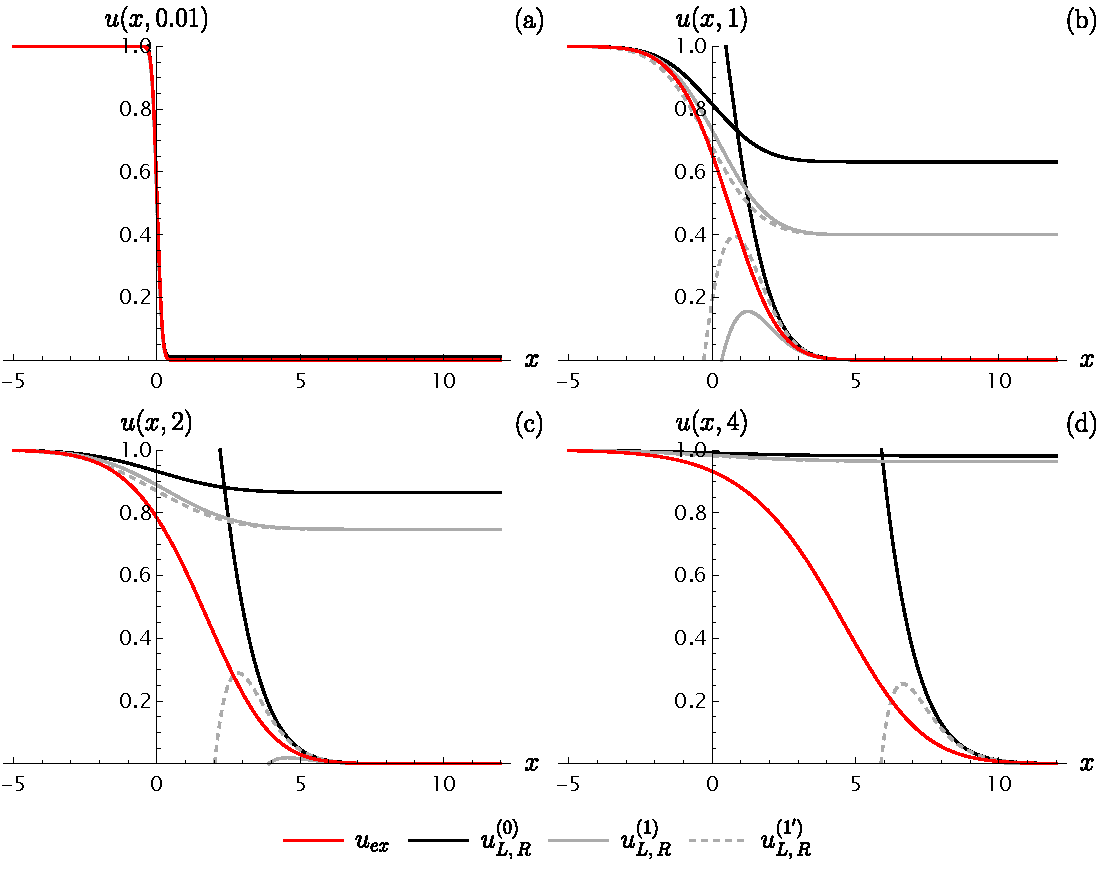
\includegraphics[width=\linewidth]{Figures/GridU1.pdf}
    \caption{BLUES approximants of the Fisher–Kolmogorov equation \eqref{eq:Fisher–Kolmogorov} with Heaviside initial condition for left \eqref{eq:linear_operator_Left} and right \eqref{eq:linear_operator_Right} Linear PDEs compared with the exact numerical solution for four different values of time $t=0.01,\, 1,\, 2$ and $4$.}
    \label{fig:GridU1}
\end{figure}
In Figure \ref{fig:GridU1} the zeroth and first BLUES approximants for the right and left problem are plotted for different values of time. Also the numerical solution is drawn in red. One observes that indeed the left and right boundary conditions are satisfied respectively for the left and right problem. Furthermore, notice that the right zeroth BLUES iterated approximant $u^{(0)}_R$ intersects with the left zeroth BLUES iterated approximant $u^{(0)}_L$ and first BLUES iterated approximant $u^{(1^\prime)}_L$. Hence, these intersections $k(t)$ present a natural point to construct a piecewise approximant to the exact wavefront solution of the Fisher–Kolmogorov equation. The result of such a construction can be seen in Figure \ref{fig:PiecewiseApproxGrid}. In particular, if one considers the left and right zeroth BLUES iterated approximants $u^{(0)}_{L,R}$ with their intersection $k_0(t)$ one can compose
\begin{align}
    u_0(x,t)\equiv
    \begin{cases}
    u^{(0)}_{L}(x,t) \qq{for} x\leq k_0(t),\\
    u^{(0)}_{R}(x,t) \qq{for} x>k_0(t),
    \end{cases}
    \qq{with} k_0(t) = 2\sqrt{t}\erfc^{-1}\left(\frac{2}{1+e^{t}}\right).
\end{align}
From Figure \ref{fig:GridU1}, one sees that if one exchanges $u^{(0)}_{L}$ with a higher iterated BLUES function of the left problem, e.g $u^{(1)}_{L}$ or $u^{(1^\prime)}_{L}$, we can construct similar wavefront approximants, respectively $u_1$ and $u_{1^\prime}$.
\begin{figure}[t]
    \centering
    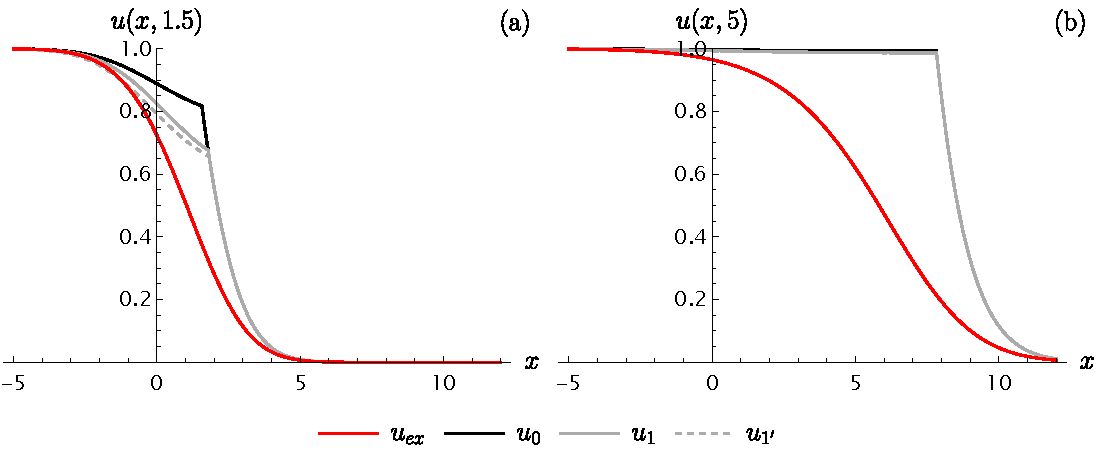
\includegraphics[width=\linewidth]{Figures/PiecewiseApproxGridAlt.pdf}
    \caption{Caption}
    \label{fig:PiecewiseApproxGrid}
\end{figure}
\section{The approximant}\label{sec:The_approximant}

In section \ref{sec:constructing_approximant}, we discussed that a proper approximant wavefront must have three vital properties: it respects the boundary conditions, the shape remains the same with respect to time and it has a constant velocity with respect to time. We will show that these properties are fulfilled for the approximants $u_0$, $u_1$ and $u_{1^\prime}$. First of all, as the wavefront approximants are composed out of constituent where the boundary conditions are respected, the first condition is indeed satisfied. Naturally, this can be ascribed to the choice of linear PDEs \eqref{eq:linear_operator_Left} and \eqref{eq:linear_operator_Right} where the BLUES approximant are constructed from. Next, to examine the fixed shape with respect to time, one could contemplate the error $\epsilon_i$ of the wavefront approximant with respect to the exact solution $u_{ex}$, given by
\begin{align}\label{eq:Error}
    \epsilon_i(t) \equiv \int_{-\infty}^{+\infty}  \abs{u_{ex}-u_i}^2\dd{x},
\end{align}
with $i\in \{0,1,1^\prime \}$. In view of the fact that we know that the exact solution evolves into wavefront which form remain constant in time, the error has also converge to a constant value in time. Indeed, in Figure \ref{fig:ErrorVelocityGrid}(a) one observes that this is the case. 
\begin{figure}[!ht]
    \centering
    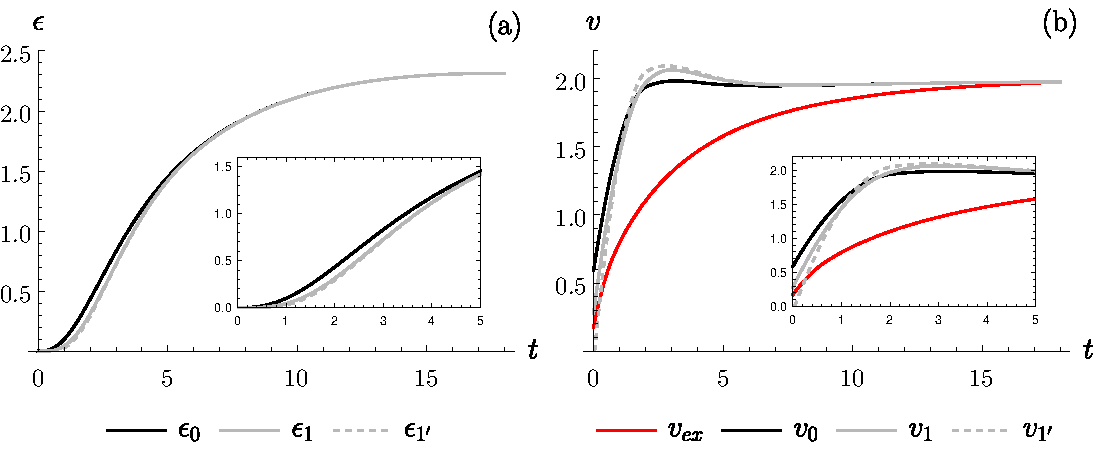
\includegraphics[width=\linewidth]{Figures/ErrorVelocityGrid.pdf}
    \caption{(a) The error defined in \eqref{eq:Error} for the three wavefront approximants $u_0$, $u_1$ and $u_1^\prime$. (b) The velocity determined with the Gibbs dividing surface method \eqref{eq:Gibbs_dividing_surface} of the wave front approximant compared with exact solution of the Fisher–Kolmogorov equation with Heaviside initial condition. }
    \label{fig:ErrorVelocityGrid}
\end{figure}

At last, one must validate the velocity of the wavefront approximants. At early times, both the wavefront approximants and the exact solution are still evolving in a traveling wave. Hence, the velocity at these times is arbitrary as it will be different for the different positions. To still have a reference point at these times one could define the velocity with a technique used in interface physics called the Gibbs dividing surface \cite{gibbs1928collected,Lamorgese2017}. The method defines a collective coordinate $\tilde{x}(t)$ of the wave-guide as a cut of a Heaviside which has the same surface area as the wavefront, i.e. by
\begin{align}\label{eq:Gibbs_dividing_surface}
    \int_{a(t)}^{b(t)}  \Theta(\tilde{x}(t)-x)-u(x, t)\dd{x}  =0.
\end{align}
The boundaries of the surface area, $a(t)$ and $b(t)$, are taken to be the position where the wavefront is significantly close to $u=1$ at the left and significantly close to $u=0$ at the right. In our case $b(t)$ can be taken infinity. After determining the collective coordinate $\tilde{x}(t)$, the velocity is defined as $v\equiv \dv*{\tilde{x}}{t}$. In Figure \ref{fig:ErrorVelocityGrid}(b) one finds the velocities for both the exact solution and the wavefront approximants. All of the velocities converge the the constant value $v=2$. This was to be suspected as velocities of the wavefront approximants at late times are completely determined by the right zeroth BLUES iteration $u^{(0)}_R$ which is just the solution of the right linear PDE \eqref{eq:linear_operator_Right}. This linear PDE captures the traveling waves behavior around the source $u=0$ and thus also the velocity of the nonlinear wavefront.



\section{Conclusions}
\lipsum[2-3]
\label{sec:conclusions}
\cleardoublepage
\appendix
\section{Details of the calculations}
\label{sec:Details_of_the_calculculations}
\begin{align}
    u^{(1)}_R = \frac{1}{4} e^t \erfc\left(\frac{x}{2 \sqrt{t}}\right)^2-\frac{1}{4} e^{2 t} \erfc\left(\frac{x}{2 \sqrt{t}}\right)^2+\frac{1}{2} e^t \erfc\left(\frac{x}{2 \sqrt{t}}\right)
\end{align}
\begin{multline}
    u^{(1)}_b 
   =1-e^{-t}+\frac{e^{-2 t}}{4}+\frac{e^{-3 t}}{4}-e^{-t} \erf\left(\frac{x}{2 \sqrt{t}}\right)+\frac{1}{2} e^{-2 t} \erf\left(\frac{x}{2 \sqrt{t}}\right)\\+\frac{1}{4} e^{-2 t} \erf\left(\frac{x}{2 \sqrt{t}}\right)^2-\frac{1}{4} e^{-3 t} \erf\left(\frac{x}{2 \sqrt{t}}\right)^2.
\end{multline}

\begin{figure}[!h]
    \centering
    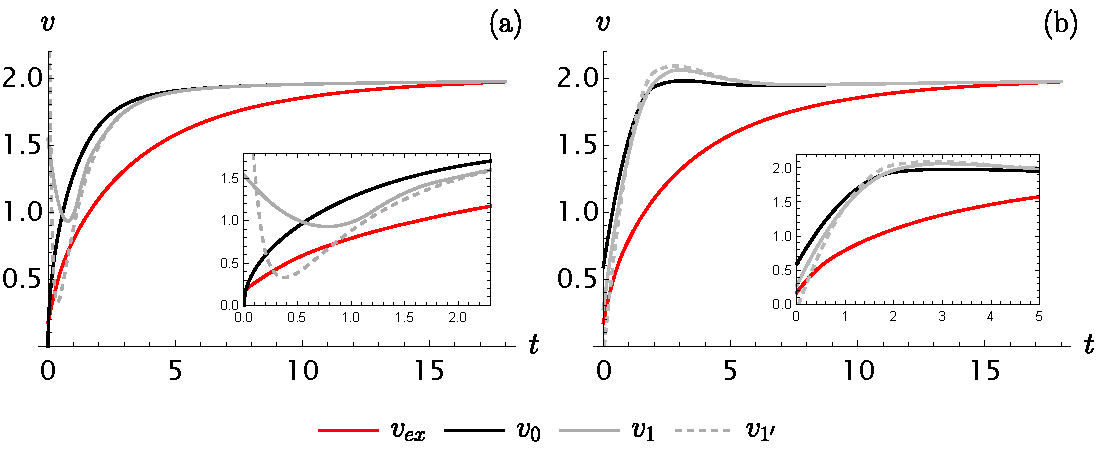
\includegraphics[width=\linewidth]{Figures/VelocityMethodsGrid.pdf}
    \caption{(a) (b) }
    \label{fig:VelocityMethodsGrid}
\end{figure}

\section{Other methods}\label{sec:Other_Methods}
\bibliography{BLUES.bib}
\end{document}